\section{Vue globale}
Voici un diagramme qui représente les différents composants de vigilate.
\begin{figure}[H]
  \caption{Diagramme de composants}
  \centering
  \vspace*{0.5cm}
  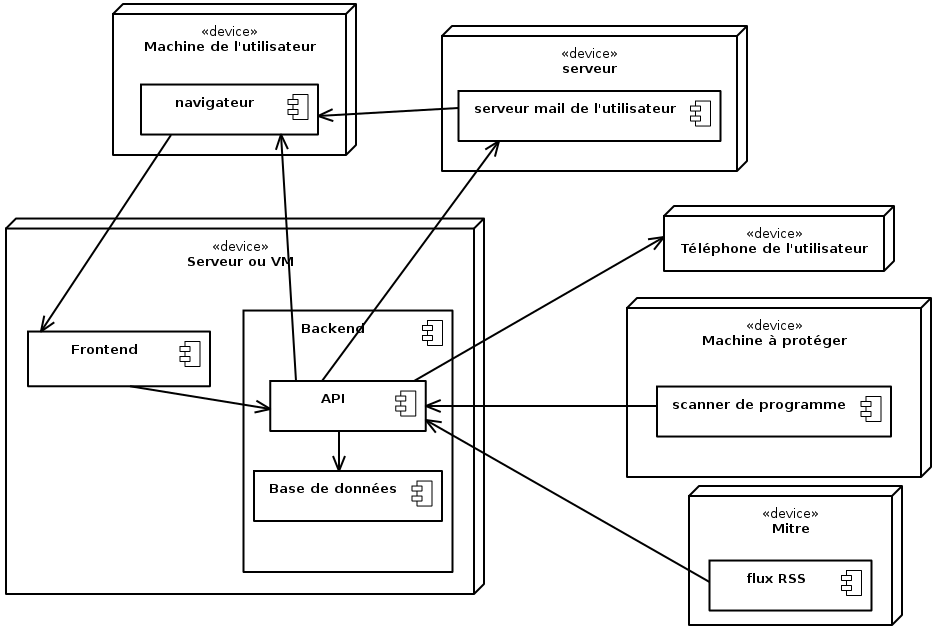
\includegraphics[width=15cm]{composants.png}
\end{figure}
\section{Composants principaux}

Un certain nombre de composants présent dans le diagramme ci-dessus existe déjà : le navigateur, le téléphone, le serveur mail et le flux RSS de mitre. Nous allons donc utiliser ces composants dans l’état dans lequel ils existent aujourd’hui.\\
Le navigateur servira à accéder au frontend pour paramétrer la solution ainsi qu’as recevoir les alertes levés par le backend (directement sur le navigateur ou via un email envoyé lui aussi par le backend).
Le serveur de mail servira juste à recevoir les emails d’alerte envoyé par le backend.\\
Le téléphone ne servira lui aussi qu’as recevoir les alertes, cette fois via un SMS.\\
Le flux RSS de mitre sert à recevoir les informations des nouvelles vulnérabilités découvertes.\\
Pour ce qui est des composants restants, à savoir le frontend, le backand (api et base de données) ainsi que le scanner de programmes, nous allons devoir les développer.\\
Le frontend serviras d’interface pour l’utilisateur afin de pouvoir paramétrer la solution Vigilate.\\
Le backend auras pour rôle de récupérer les informations sur les nouvelles vulnérabilités et la liste des programme installé ainsi que de lever des alertes de sécurité lorsqu’un utilisateur est vulnérable. Le backend utilise les paramètre entré par l’utilisateur pour savoir si une alerte doit être levé et par quel moyen.\\
Le scanner de programme sert à faciliter l’utilisation de Vigilate, en effet, il permet à l’utilisateur de mettre à jour automatiquement la liste des programmes installer sans avoir à les ajouter tous à la main via le frontend.\\
